\documentclass[aspectratio=169, 12pt]{beamer}
% Note: You can use the handout mode by changing to [aspectratio=169, 12pt, handout]. This results in the pauses being removed.

\newcommand{\handout}{false}
% This command excludes certain frames when the boolean is set to true.

\usepackage{algorithm}
\usepackage{algpseudocode}
\usepackage{amsmath}
\usepackage{amsthm}
\usepackage{blindtext}	% TODO Remove
\usepackage{changes}
\usepackage[nameinlink,capitalise]{cleveref}
\usepackage{enumitem}
\usepackage{amsbsy}
\usepackage{afterpage}
\usepackage{hyperref}
\usepackage[acronym]{glossaries} % toc does not work properly
\usepackage{siunitx}
\usepackage{subcaption} 
\usepackage{thmtools}
\usepackage{tikz}

\usetikzlibrary{automata,arrows,shapes}

\makeglossaries

\graphicspath{{./figures/}}

%% Glossary and Acronyms %%
%% List of acronyms %%
% Reference definition:
% - \newacronym[options]{label}{short}{long}
%	options: description, longplural, ...
%
% Reference usage:
% - \acrlong{label}  : displays the full text of the acronym
% - \acrshort{label} : displays the abbreviation
% - \acrfull{label}  : displays the full text followed by the abbreviation
% - \acrshortpl{label} : the plural of the abbreviation (similarly for acrlongpl and acrfullpl)

\newacronym{acr:dtp}{DTP}{Decision-Theoretic Planning}

\newacronym{acr:hmm}{HMM}{Hidden Markov Model}

\newacronym[longplural=Markov Decision Processes]{acr:mdp}{MDP}{Markov Decision Process}

\newacronym{acr:pomdp}{POMDP}{Partially Observable \acrshort{acr:mdp}}

\newacronym{acr:sdm}{SDM}{Sequential Decision Making}
%% Glossary Entries:
%
% Reference definition:
% \newglossaryentry{maths}
% {
% 	name=mathematics,
% 	description={Mathematics is what mathematicians do}
% }
%
% Reference usage:
% - \gls{ } Prints term lower case
% - \Gls{ } Prints term upper case
% - \glspl{ } Prints term plural lower case
% - \Glspl{ } Prints term plural upper case

\newglossaryentry{maths}{
	name={mathematics},
	description={Mathematics}
}

\newcommand\mat[1]{\pmb{#1}}
\newcommand\arr[1]{\pmb{#1}}
\DeclareMathOperator*{\argmax}{arg\,max}

%% Custom Definitions %%
\def\subsubsectionautorefname{Section}
\def\subsectionautorefname{Section}
\def\sectionautorefname{Section}
\def\chapterautorefname{Chapter}
\def\algorithmautorefname{Algorithm}

%\declaretheoremstyle[bodyfont=\normalfont]{normalbody}
%\declaretheorem[style=normalbody,name=Definition]{definition}
\theoremstyle{definition}
\newtheorem{definition}{Definition}
\newtheorem*{problem}{Problem Statement}

%% Pseudocode settings %%
\newcommand*\Let[2]{\State #1 $\gets$ #2}
\algrenewcommand{\algorithmiccomment}[1]{\hfill$\rhd$ #1} % Fix for comments in pseudocode

%% Title and Cover Pages %%

%% Use Roman numerals for the page numbers of the title pages and table of
%% contents.
\frontmatter

%% Uncomment following 16 lines for a cover with a picture on the lower half only
\title[tudelft-white]{Learning and Optimizing Probabilistic Models for Planning Under Uncertainty} %in Mobile Robot Navigation}
%\subtitle[tudelft-black]{Optional subtitle}
\author[tudelft-white]{R. van Bekkum}
\affiliation{Delft University of Technology}
\coverimage{figures/tank.jpg}
\covertext[tudelft-white]{
	\textbf{Cover Text} \\
	possibly \\
	spanning 
	multiple 
	lines
	\vfill
	ISBN 000-00-0000-000-0
}
\setpagecolor{tudelft-cyan}
%\makecover[split]

% TEMPORARY
\newcommand{\showoutline}[1]{
	\vspace{0.3cm}
	\hrule
	\vspace{0.3cm}
	{\large\textbf{PLANNED OUTLINE}:}
	\vspace{0.3cm}
	\hrule
	\vspace{0.3cm}
	{#1}
	\vspace{0.3cm}
	\hrule
	\vspace{0.3cm}	
}

\title{Learning and Optimizing Probabilistic Models for Planning under Uncertainty}
%\titlegraphic{{\vspace{-4pt}\setlength{\fboxsep}{0pt}\setlength{\fboxrule}{1pt}\fbox{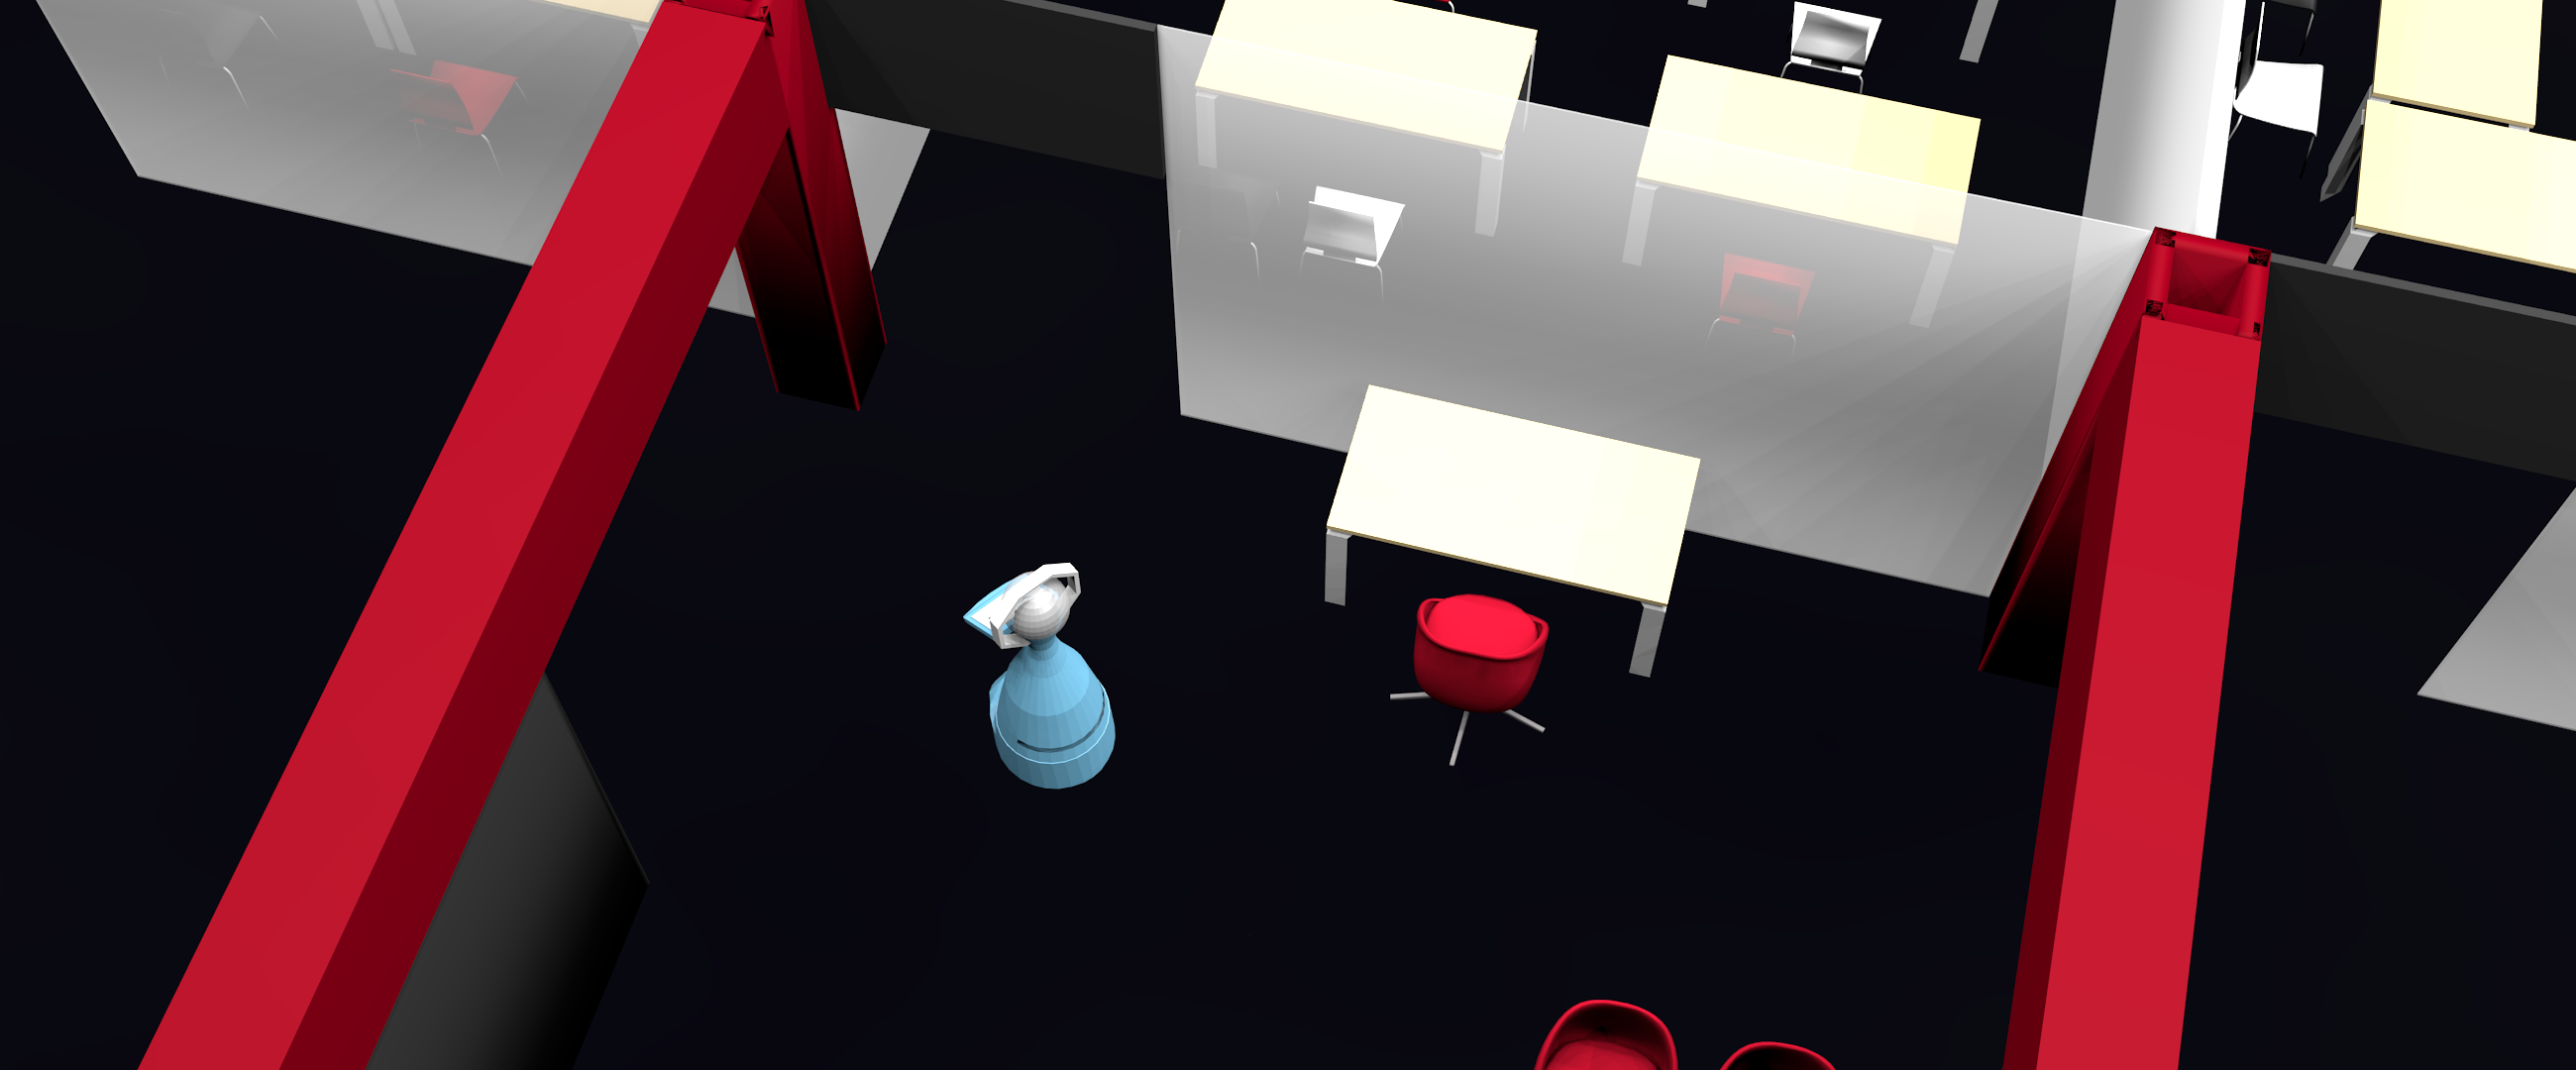
\includegraphics[width=0.35\textwidth]{figures/render_4}}\vspace{-10pt}}}
\author{R. van Bekkum}
\institute{Faculty of Electrical Engineering, Mathematics and Computer Science \\ Delft University of Technology}

\date{September 27, 2017}

\begin{document}

\begingroup
\setbeamertemplate{headline}{%
	\leavevmode%
	\hbox{%
		\begin{beamercolorbox}[wd=\paperwidth,ht=2.5ex,dp=1.25ex]{palette tertiary}%
		\end{beamercolorbox}%
	}
}

% Title Sheet
\frame{\titlepage}

\endgroup %TODO Add outline?

\section{Background and Problem}

\begin{frame}
	\frametitle{Planning under Uncertainty}
	\framesubtitle{Domain Characteristics}
	
	\begin{columns}[T]
		\begin{column}{.7\textwidth}
			\begin{itemize}
				\item A system is controlled by one or more \textit{agents}
				\item \textit{Uncertain domain dynamics}, i.e.\\ uncertainty may be present in:
				\begin{itemize}
					\item Execution of actions (e.g., robot may slip)
					\item Exogenous factors (e.g., doors open/closed)
					\item Percepts (e.g., sensor noise)
				\end{itemize}
				\item \textit{Sequential decision making}
				\begin{itemize}
					\item Non-myopic agents
					\item Selection of actions with high future pay-off
				\end{itemize}
			\end{itemize}
		\end{column}
		\begin{column}{.35\textwidth}
		%	%\vspace{-30pt}
			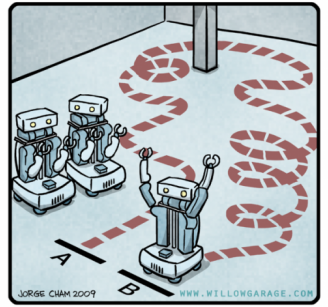
\includegraphics[width=1.0\textwidth, right]{figures/path-planning2}
		\end{column}
	\end{columns}
\end{frame}

\begin{frame}
	\frametitle{Planning under Uncertainty}
	\framesubtitle{Example Domains}
	
	\begin{columns}[t]
		\begin{column}{.3\textwidth}
			\centering 
			\begin{overlayarea}{\linewidth}{4.75cm}
				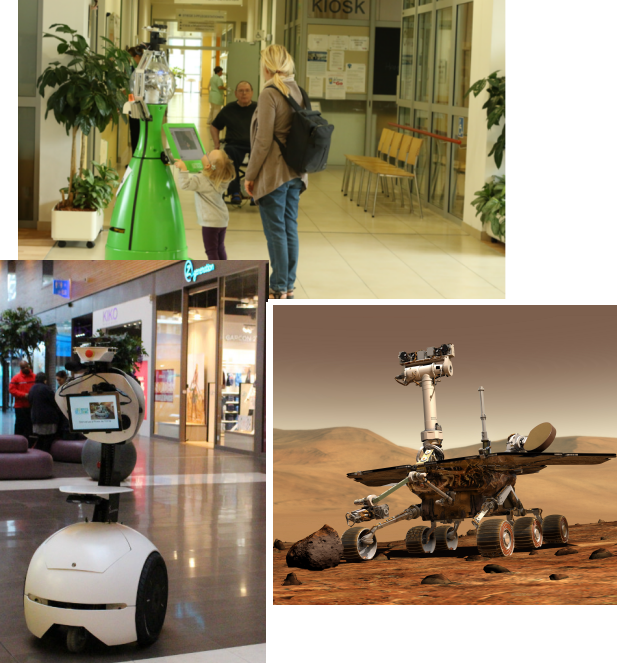
\includegraphics[width=\columnwidth]{figures/path-planning}
			\end{overlayarea}
			\captionof*{figure}{\scriptsize\textit{\textcolor{tudBlack}{Path planning}}}
		\end{column}
		\begin{column}{.25\textwidth}
			\centering
			\begin{overlayarea}{\linewidth}{4.75cm}
				\centering
				\vspace{-18pt}
				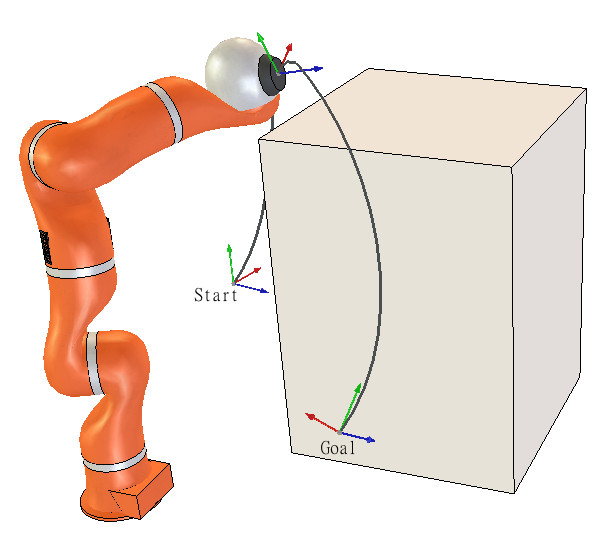
\includegraphics[width=0.75\columnwidth]{figures/motion-planning}\\
				{\scriptsize\textit{Motion planning}}\\\vspace{6pt}
				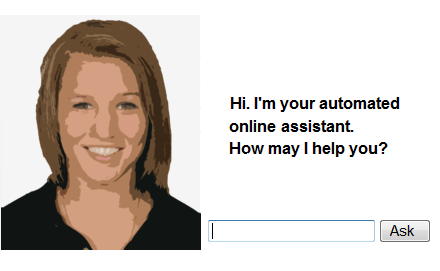
\includegraphics[width=0.85\columnwidth]{figures/dialog_system_2}
			\end{overlayarea}
			\captionof*{figure}{\scriptsize\textit{\textcolor{tudBlack}{Dialog Management}}}
		\end{column}
		\begin{column}{.3\textwidth}
			\centering
			\begin{overlayarea}{\linewidth}{4.75cm}
				\vspace{0pt}
				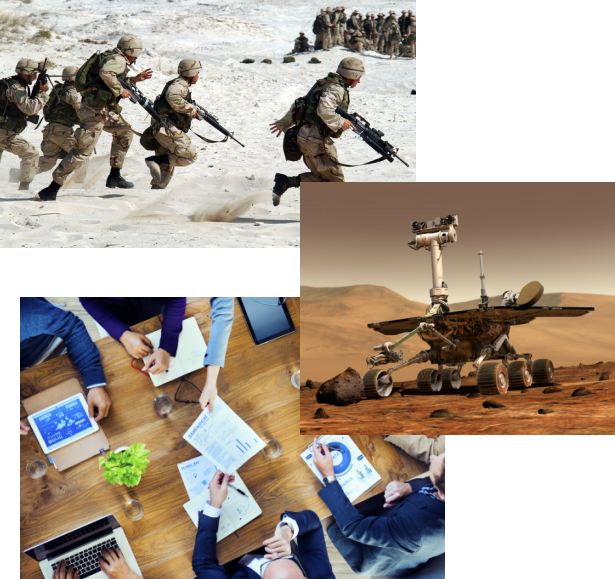
\includegraphics[width=\columnwidth]{figures/operations-planning5}
			\end{overlayarea}
			\captionof*{figure}{\scriptsize\textit{\textcolor{tudBlack}{Operations planning}}}
		\end{column}
	\end{columns}
	\imgsrc*[Image credits]{Hawes et al. \cite{hawes2016strands}, \href{https://coaches.greyc.fr}{Iocchi et al.} \cite{iocchi2016practical}, \href{http://www.coppeliarobotics.com/helpFiles/en/motionPlanningModule.htm}{V-REP Manual}, Bemidji State University}
\end{frame}
% Examples Operations Planning:
% - Military Operations Planning: Decision-Theoretic Military Operations Planning
% - Markov Decision Processes in AI: (Operations Planning Rover Exploration) https://www.safaribooksonline.com/library/view/markov-decision-processes/9781118620106/xhtml/Chapter15.html
% - Project Management: Engineering the Decision-Making Process Using Multiple Markov Theories and DEMO
\imgsrc*{off}

\begin{frame}
	\frametitle{Planning under Uncertainty}
	\framesubtitle{Typical Development Routine}
	\centering
	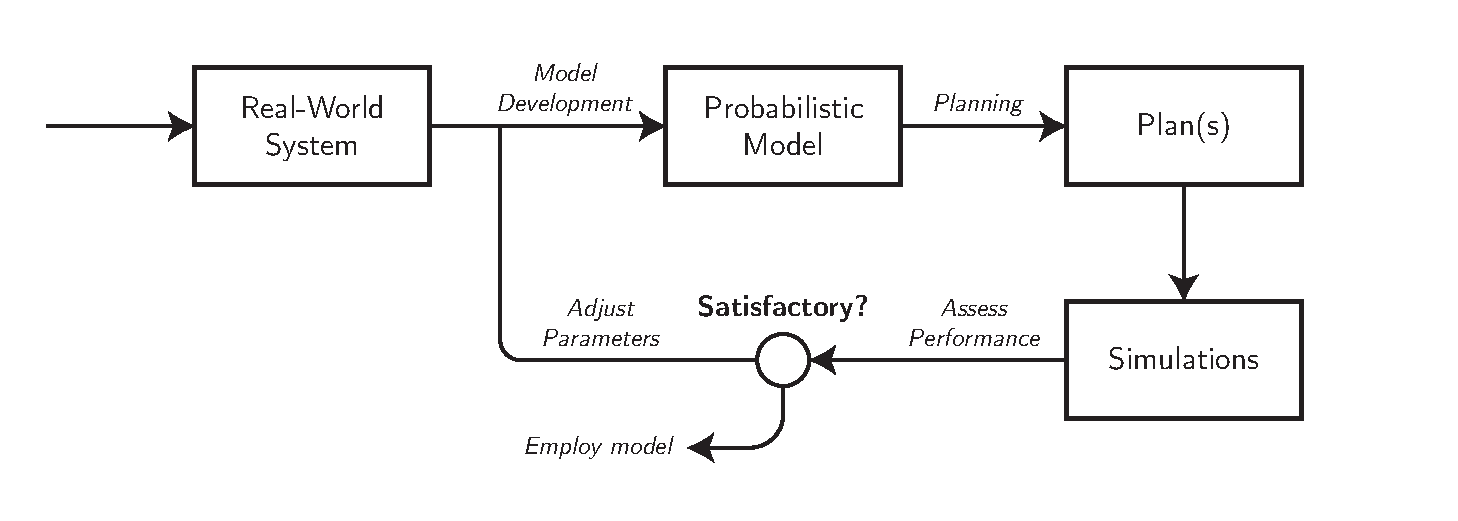
\includegraphics[width=\textwidth]{figures/high-level-planning-diagram}
\end{frame}

\begin{frame}
	\frametitle{Planning under Uncertainty}
	\framesubtitle{Markov Decision Processes (MDPs)}
	
	In DTP systems are modeled by probabilistic models, e.g. MDPs:
	\begin{columns}[T]
		\begin{column}{0.6\textwidth}
			\begin{definition}
				An MDP is a 5-tuple $\mathcal{M} = (\mathcal{S}, s_0, A, \delta, R)$:
				\begin{itemize}
					\item $\mathcal{S}$ is the state-space, $s_0 \in \mathcal{S}$ the initial state
					\item $A$ is the action-space
					\item $\delta: \mathcal{S} \times A \times \mathcal{S} \mapsto [0, 1]$ is the transition function % $\delta: S \times S \times A \mapsto [0,1]$
					\item $R: \mathcal{S} \times A \times \mathcal{S} \mapsto \mathbb{R}$ is the reward function
				\end{itemize}
			\end{definition}
		\end{column}
		\begin{column}{0.425\textwidth}
			\vspace{26pt}
			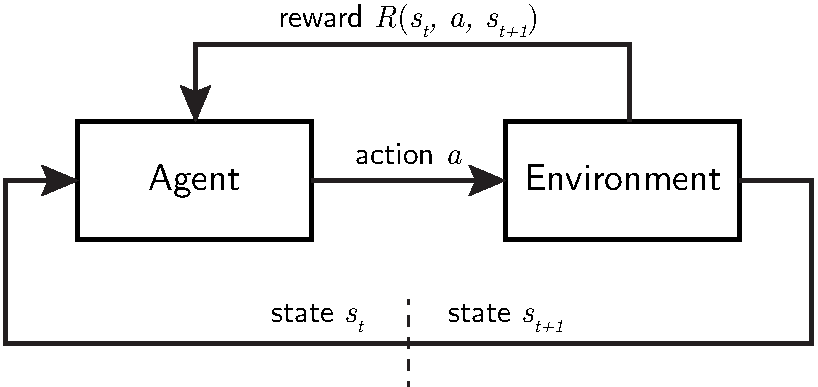
\includegraphics[width=\linewidth]{figures/mdp-2v2}
		\end{column}
	\end{columns}
\end{frame}

\begin{frame}
	\frametitle{Planning under Uncertainty}
	\framesubtitle{Planning with MDPs}
	\begin{center}
	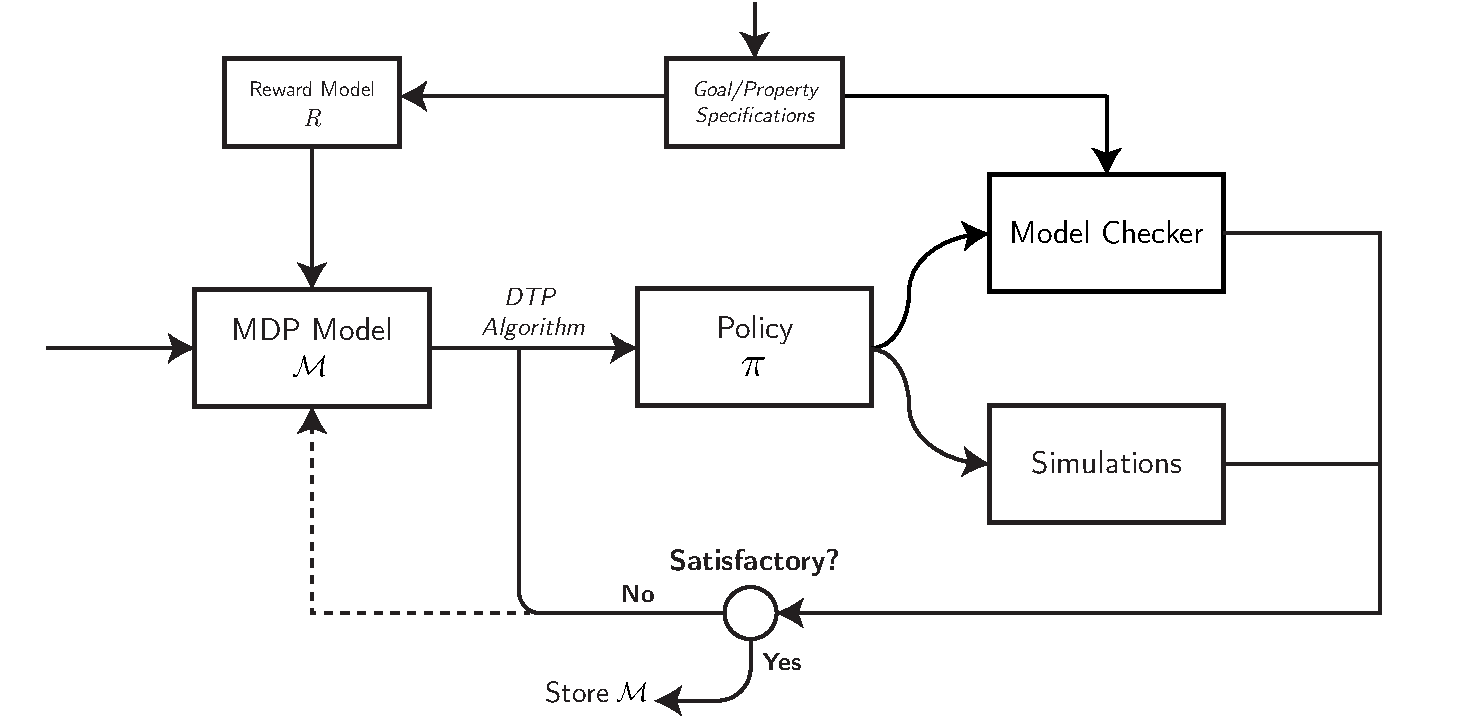
\includegraphics[width=0.9\textwidth]{figures/mdp-planning-diagram-v32-cropped}
\end{center}
\end{frame}

\begin{frame}
	\frametitle{Planning under Uncertainty}
	\framesubtitle{Model Development}
	
	\textcolor{tudBlack}{\textbf{Problem:}} How to obtain a suitable MDP for offline planning?
	\pause
	\vfill
	\textcolor{tudBlack}{\textbf{Classical approach:}} Model development by a \textit{human designer}, however:
	\begin{itemize}
		\item Requires significant effort (e.g., trial-and-error)
		\item Typically demands knowledge/experience, accompanied by high costs
	\end{itemize}
	\pause
	\vfill
	\textcolor{tudBlack}{\textbf{Alternative:}} Use Reinforcement Learning instead of Planning, however:
	\begin{itemize}
		\item Requires direct interaction with environment %(slow in complex dynamic environment) % (chance of errors)
		\item One might require \textit{reusable} models, applicable for multiple tasks % You do have model-based RL, but we might want a model that generalizes for multiple tasks
		%\item Still requires definition of state-spaces (and actions and rewards)
	\end{itemize}
\end{frame}

\begin{frame}[t]
	\frametitle{Planning under Uncertainty}
	\framesubtitle{Model Development}
	\vspace{8pt}
	\textcolor{tudBlack}{\textbf{Problem:}} How to obtain a suitable MDP for offline planning?\\
	\vspace{14pt}
	\textcolor{tudblue}{\textbf{Idea:}} Automate the model development process \\through learning algorithms 
	\begin{itemize}
		\item Learn from (exploration) data about the environment
		\item Optimization for the best MDP model
	\end{itemize}

\end{frame}

\begin{frame}
\frametitle{Problem Description}
\framesubtitle{Problem Statement}



\end{frame}

\begin{frame}
\frametitle{Problem Description}
\framesubtitle{Related Work}



\end{frame}

\begin{frame}
\frametitle{Problem Description}
\framesubtitle{Research Questions}

\begin{block}{Main Research Question}
%	How can the task of learning a \textit{performance-maximizing} MDP from a dataset be automated?
How can the task of obtaining an MDP that maximizes the yielded performance of executing plans that are derived from it, given a dataset about the system under consideration, be automated? %TODO Probably too long text, use shorter version?
\end{block}

\end{frame}

\section{Optimization Framework}

\setbeamercovered{transparent}
\begin{frame}[t]
\frametitle{Proposed Solution}
\framesubtitle{General Idea}

\begin{itemize}
	\item<1-> Explore the hyperparameter space of model learning algorithms
	\item<2-> Use \textit{Bayesian Optimization} to sequentially sample hyperparameter~settings $\theta$ towards a global maximizer of a performance measure of learned MDPs
\end{itemize}

\begin{center}
	\includegraphics<-2>[width=\textwidth]{figures/bo_toy_example_v2_transparent}
	\includegraphics<3->[width=\textwidth]{figures/bo_toy_example_v2}
\end{center}

\end{frame}
\setbeamercovered{invisible}

\begin{frame}
\frametitle{Proposed Solution}
\framesubtitle{Running Example: Path Planning for Mobile Robot Navigation}

\centering
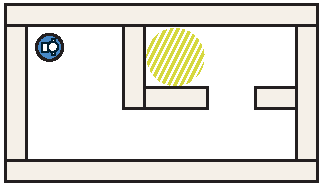
\includegraphics[width=.3\textwidth]{figures/dummy-map-2-1}
\qquad
\includegraphics<-1| handout:0>[width=.3\textwidth]{figures/dummy-map-2-2-transparent}
\includegraphics<2->[width=.3\textwidth]{figures/dummy-map-2-2v2}\\\vspace{8pt}
\includegraphics<-2| handout:0>[width=.3\textwidth]{figures/dummy-map-2-3-transparent}
\includegraphics<3->[width=.3\textwidth]{figures/dummy-map-2-3} \qquad
\includegraphics<-3| handout:0>[width=.3\textwidth]{figures/dummy-map-2-4-transparent} \includegraphics<4->[width=.3\textwidth]{figures/dummy-map-2-4}


\end{frame}

\begin{frame}
\frametitle{Proposed Solution}
\framesubtitle{Performance Measure}
\begin{itemize}
	\item<1-> \footnotesize Performance is assessed over multiple tasks $T$ (each mappable to a pair $(s_0, R)$)
	\item<2-> Based on Value Functions from DTP algorithm (e.g., VI, PI):
	$$V_{\mathit{DTP}, (s_0, R)} = V[s_0]$$
	\item<3-> Based on Simulations:
	$$V_{\mathit{SIM}, (s_0, R)} = \gamma^n \cdot R[i]$$
	\item<4-> Combined:
	$$V_{\mathcal{M}} = \frac{\sum_{t \in T_\mathcal{M}} \beta \cdot V_{\mathit{DTP}, t} + (1 - \beta) \cdot V_{\mathit{SIM}, t}}{|T_\mathcal{M}|}$$
%	% Level of abstraction
%	\item Value Function
%	\item Simulations
%	
%	\item Lorem ipsum dolor sit amet
%$$V_{\mathcal{M}} = \frac{\sum_{t \in T_\mathcal{M}} \beta \cdot V_{\mathit{DTP}, t} + (1 - \beta) \cdot V_{\mathit{SIM}, t}}{|T_\mathcal{M}|}$$
\end{itemize}

\end{frame}

\begin{frame}
\frametitle{Proposed Solution}
\framesubtitle{Base Framework}
	\vspace{-10pt}
	\begin{center}
		\includegraphics<1| handout:0>[width=1\textwidth]{figures/optimization-routine/learning-cycle-1.pdf}
		\includegraphics<2| handout:0>[width=1\textwidth]{figures/optimization-routine/learning-cycle-2.pdf}
		\includegraphics<3| handout:0>[width=1\textwidth]{figures/optimization-routine/learning-cycle-3.pdf}
		\includegraphics<4| handout:0>[width=1\textwidth]{figures/optimization-routine/learning-cycle-4.pdf}
		\includegraphics<5>[width=1\textwidth]{figures/optimization-routine/learning-cycle-5.pdf}
	\end{center}
\end{frame}

\begin{frame}
\frametitle{Proposed Solution}
\framesubtitle{Base Framework}
	\vspace{-10pt}
	\begin{center}
		\includegraphics<1| handout:0>[width=1\textwidth]{figures/optimization-routine/learning-cycle-simplified-1.pdf}
		\includegraphics<2| handout:0>[width=1\textwidth]{figures/optimization-routine/learning-cycle-simplified-2.pdf}
		\includegraphics<3>[width=1\textwidth]{figures/optimization-routine/learning-cycle-simplified-v2-3.pdf}
	\end{center}
\end{frame}

\begin{frame}
\frametitle{Proposed Solution}
\framesubtitle{Multi-Phase Framework: Phase 1}

\begin{center}
	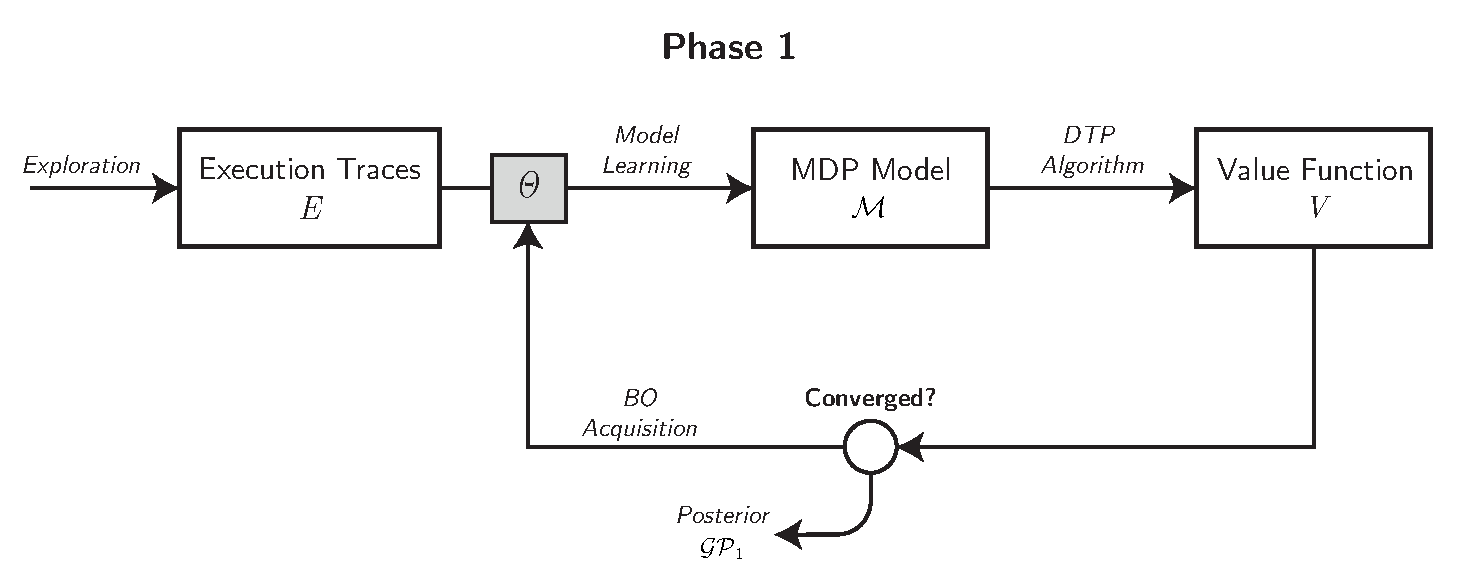
\includegraphics[width=\textwidth]{figures/phase-1v2}
\end{center}

\end{frame}

\begin{frame}
	\frametitle{Proposed Solution}
	\framesubtitle{Multi-Phase Framework: Phase 2}
	
	\begin{center}
		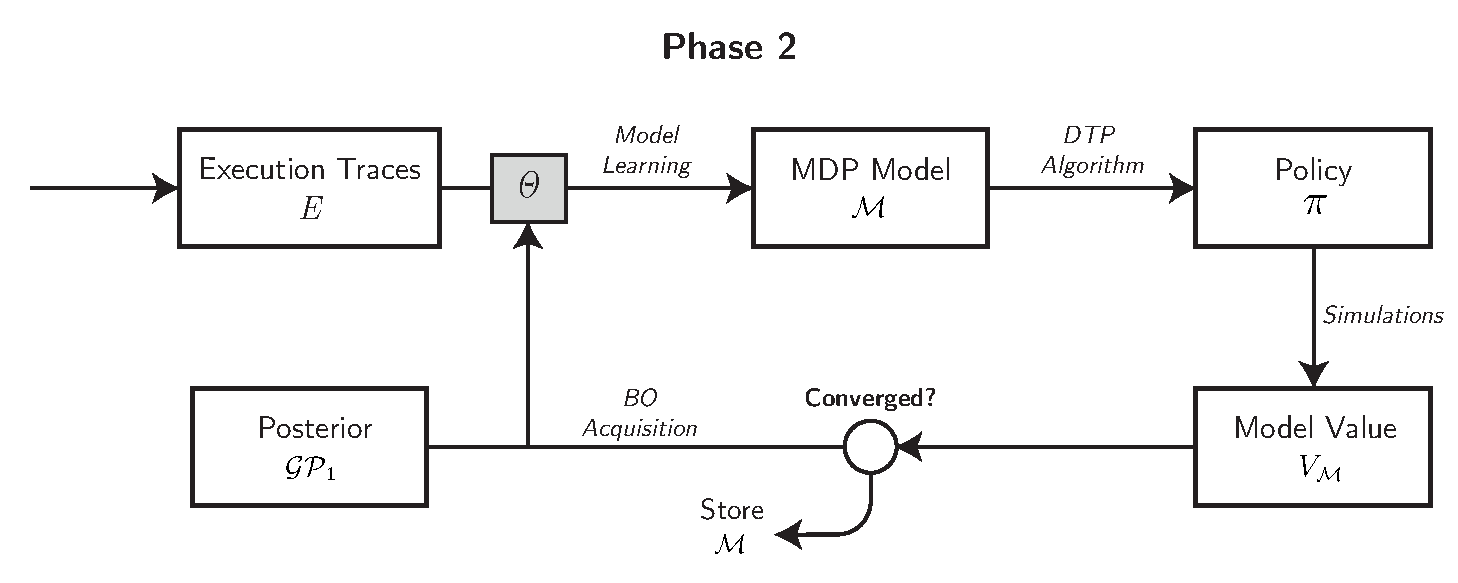
\includegraphics[width=\textwidth]{figures/phase-2v3}
	\end{center}
	
\end{frame}

\begin{frame}
	\frametitle{Proposed Solution}
	\framesubtitle{Multi-Phase Framework: Phase 3}
	
	\begin{center}
		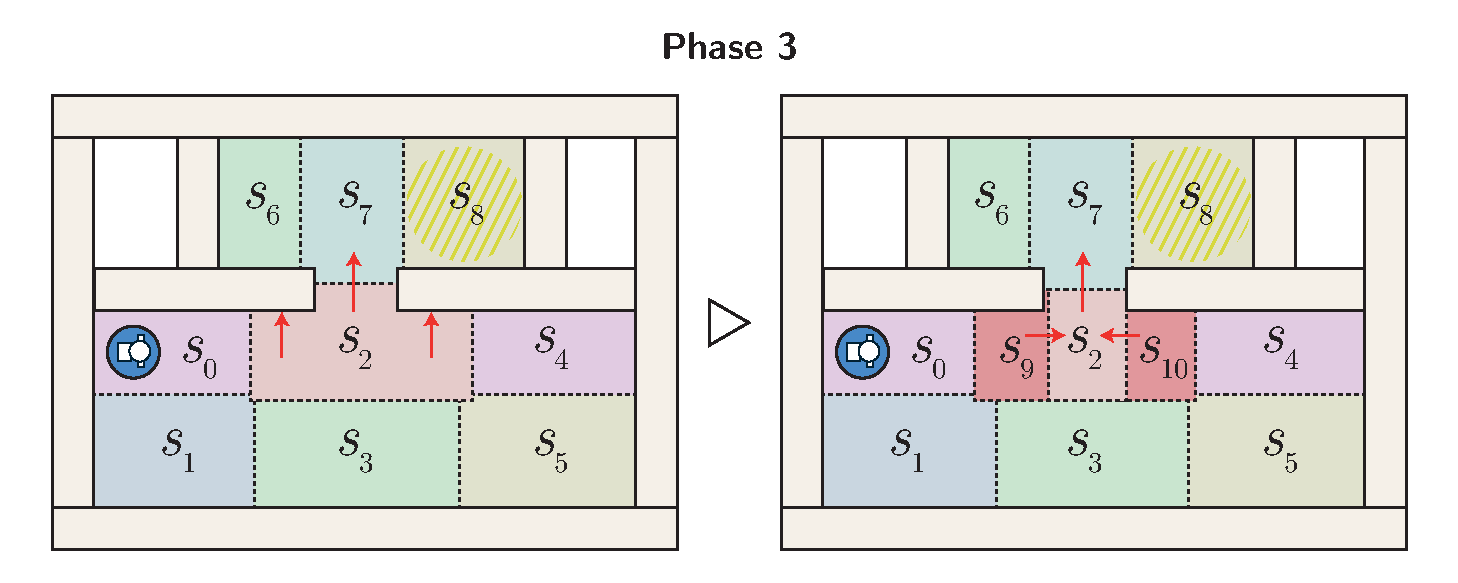
\includegraphics[width=\textwidth]{figures/phase-3}
	\end{center}
	
\end{frame}

\section{Experimental Results}

\begin{frame}
\frametitle{Experimental Results}

% How was our solution tested/evaluated?
% What experiments have been done?
% Which observations were made from the results?

\end{frame}

\section{Conclusions and Recommendations}

\begin{frame}
\frametitle{Conclusions and Recommendations}

%TODO

\end{frame}

\section{} % On purpose empty!

\begingroup
\setbeamertemplate{headline}{%
\leavevmode%
  \hbox{%
    \begin{beamercolorbox}[wd=\paperwidth,ht=2.5ex,dp=1.25ex]{palette tertiary}%
    \end{beamercolorbox}%
  }
}

% Title Sheet
\frame{\titlepage}

\begin{frame}[allowframebreaks]
\frametitle{References}\nocite{*}
\scriptsize
\bibliography{references}
\end{frame}

\endgroup

\bibliographystyle{abbrv}

\end{document}


